To test whether our thread library could combat head-of-line blocking in a large
system, we benchmarked
\textit{hyper}, the highest-performing Web server in TechEmpower's plaintext
benchmark as of July 2019~\cite{www-hyper}.  We built \textit{hyper} against
\textit{libturquoise} configured with a task timeout of 2 ms, give or take a
100-$\mu$s \textit{libinger} preemption interval, and configured it to serve
responses only after spinning in a busy loop for a number of iterations specified in
each request.  For our client, we modified version 4.1.0 of the
\textit{wrk}~\cite{www-wrk} closed-loop HTTP load generator to separately record the
latency distributions of two different request classes.

Our testbed consisted of two machines connected by a direct 10-GbE link.  We pinned
\textit{hyper} to the 16 physical cores on the NIC's NUMA node of our Broadwell
server.  Our client machine, a Intel Xeon E5-2697 v3 (Haswell) running Linux 4.10.0,
ran a separate \textit{wrk} process pinned to each of the 14 logical cores on the
NIC's NUMA node.  Each client core maintained two concurrent pipelined HTTP
connections.

\begin{figure*}[t]
	\begin{minipage}{\columnwidth}
	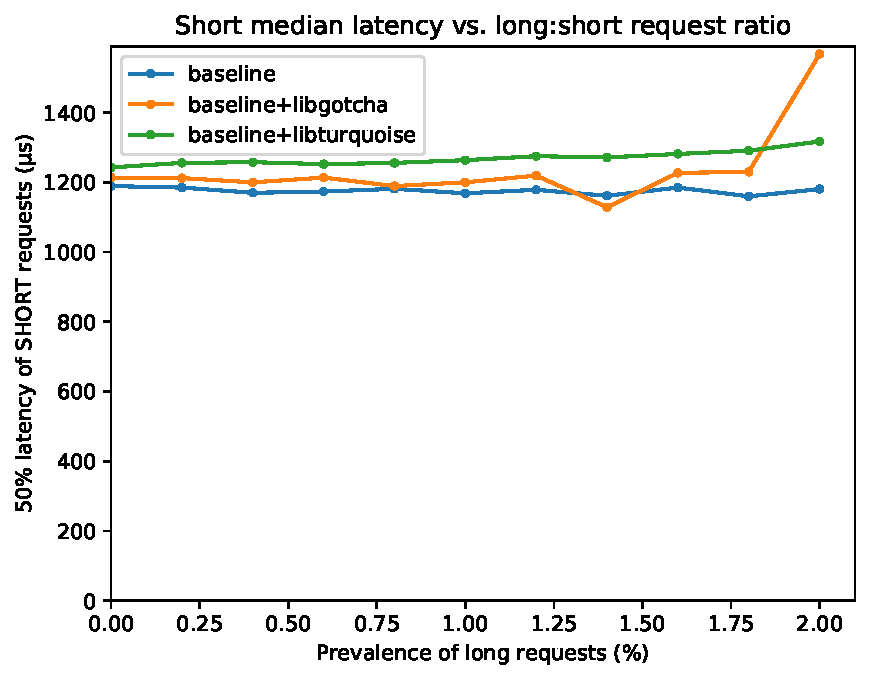
\includegraphics[width=\textwidth]{figs/twooom_50-short}
	\subcaption{Median latency}
	\end{minipage}
%
	\begin{minipage}{\columnwidth}
	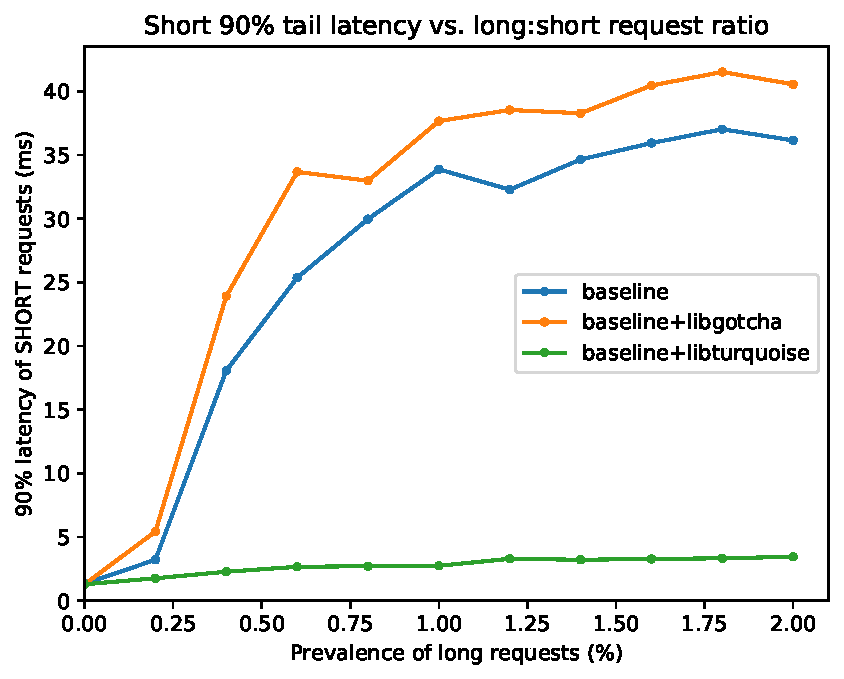
\includegraphics[width=\textwidth]{figs/twooom_90-short}
	\subcaption{90\% tail latency}
	\end{minipage}

	\begin{minipage}{\columnwidth}
	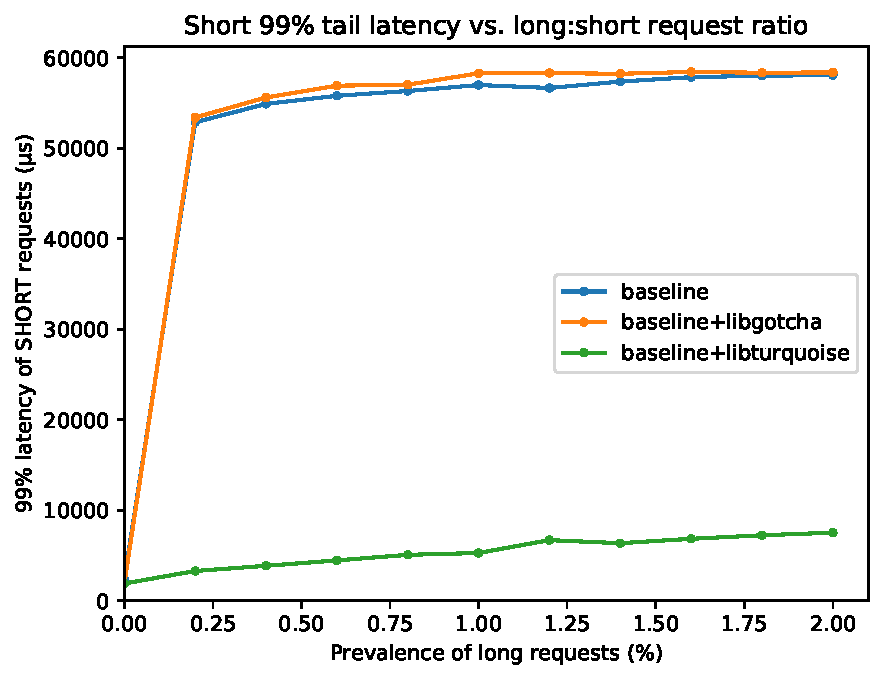
\includegraphics[width=\textwidth]{figs/twooom_99-short}
	\subcaption{99\% tail latency}
	\end{minipage}
%
	\begin{minipage}{\columnwidth}
	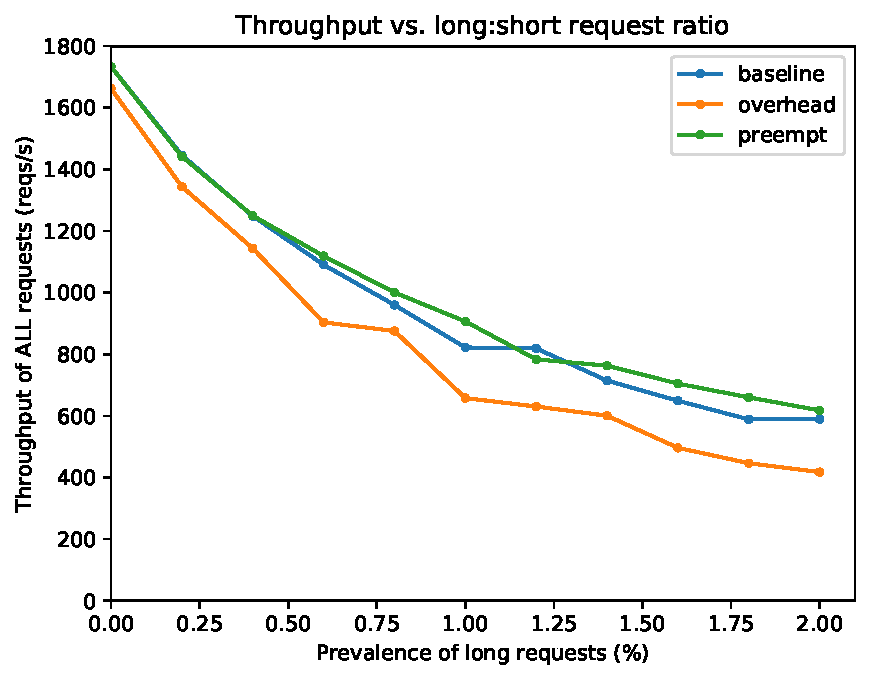
\includegraphics[width=\textwidth]{figs/twooom_tput}
	\subcaption{Overall throughput}
	\end{minipage}
\caption{\textit{hyper} Web server with 500-$\mu$s (short) and 50-ms (long) requests}
\label{fig:hyper}
\end{figure*}

We used loop lengths of approximately 500 $\mu$s and 50 ms for short and long requests,
respectively, viewing the latter requests as possible DoS attacks on the system.
We varied the percentage of long requests from 0\% to 2\% and measured the round-trip
median and tail latencies of short requests and the throughput of all requests.
Figure~\ref{fig:hyper} plots the results for three server configurations:\@
\texttt{baseline} is cooperative scheduling via \textit{tokio-threadpool},
\texttt{baseline+libgotcha} is the same but with \textit{libgotcha} loaded to assess
the
impact of slower dynamic function calls, and \texttt{baseline+libturquoise} is
preemptive
scheduling via \textit{libturquoise}.  A 2\% long request mix was enough to reduce
the throughput of the \textit{libgotcha} server enough to impact the
median short request latency.
The experiment shows that the preemptible
functions stack keeps the tail latency of short requests scaling linearly at the cost
of a
modest 4.5\% median latency overhead when not under attack.

\solb{Is it worth trying to get this running with HTTPS to increase dependence on
dynamic libraries?}
